%!TEX root = widefieldscan.tex
\svnidlong
{$HeadURL$}
{$LastChangedDate$}
{$LastChangedRevision$}
{$LastChangedBy$}

\ifhtml
\else
\begin{center}
	\fbox{
		\begin{minipage}{.618\columnwidth}
		The section below is versioned at \url{\svnkw{HeadURL}} (last commit @ \svnfileday.\svnfilemonth.\svnfileyear \space \svnfilehour:\svnfileminute, Revision: \svnkw{LastChangedRevision}).
		\end{minipage}
	} 
\end{center}
\fi

\section{Summary}
The proposed method establishes an increase of the visible FOV up to five times what is conventionally available. We have shown that we can provide different scanning protocols based on needs of the end-user of TOMCAT. The end-user has the possibility to choose a suitable scanning protocol depending on a balance between acquisition time and reconstruction quality. We managed to reduce the image acquisition time down to \SI{14}{\percent} of the comparable gold standard scan while keeping the quality of the reconstructed tomographic dataset on a level that still permitted automated segmentation of the lung structure and surrounding airspace, as shown in figure~\ref{fig:BvsT}.

Further increases of the FOV are only theoretically limited, but face problems with the amount of data to process. The dataset shown in figure~\ref{fig:LungSlabSophie} is composed of 1024 tiff-Files each with a size of 4852\(\times\)4852 pixels, which adds up to a total size of nearly \SI{23}{\giga B}. Calculations and visualizations of datasets of this size require great optimizations of the processing queue and automation of calculations\todo{elaborate a bit more\ldots}.

The stitching of the multiple overlapping projections has been automated using custom made MATLAB scripts and will be implemented at the beamline for end-user access. Since the stitching of the overlapping subscans is quite a time-consuming process it would be desirable to directly implement the stitching in to the present sinogram generation routines. This would also reduce the load on the file server, since at the moment, all the projection from the subscans are read from disk, merged to big projections and these big projections is then subsequently written to disk. If would be desirable to directly generate merged sinograms from the overlapping subscans to define the reconstruction parameters and then perform the merging and reconstruction on the cluster without intermediate merging step\todo{Is this planned? Or is this too far-fetched for TOMCAT-team?}.

\section{Outlook}
\label{sec:outlook}
The wide field scanning method has been developed to enable the high-resolution tomographic imaging of entire acini, something which would not have been possible with the  ``simple'' tomographic imaging method present at TOMCAT.

In addition to the multiple scans of the same sample to assess the method, we also recorded tomographic datasets with increased FOV from distal-medial edges of right lower lung lobes of Sprague Dawley rats obtained at post-natal days 4, 10, 21, 36 and 60. With these samples we have begun to study the skeleton of the terminal airways to quantitatively differentiate the lung development at this post-natal stage\todo{add manuscript in preparation?}.

Figure~\ref{fig:skel} shows a three dimensional visualization of such a lung lobe including the extracted segments and the airway skeleton of such a segment. We are currently analyzing the skeletons of the terminal airways at different stages in lung development and plan to publish the morphological details as soon as possible.

\renewcommand{\imsize}{\linewidth}
\pgfmathsetlength{\imagewidth}{\imsize} % desired displayed width of image
\pgfmathsetlength{\imagescale}{\imagewidth/1520} % pixel width of imagefile used below
\begin{figure}
	\centering
	\begin{tikzpicture}[x=\imagescale,y=-\imagescale]
		\def\x{950}
		\def\y{725}
		\node[anchor=north west,inner sep=0pt,outer sep=0pt] at (0,0)
		{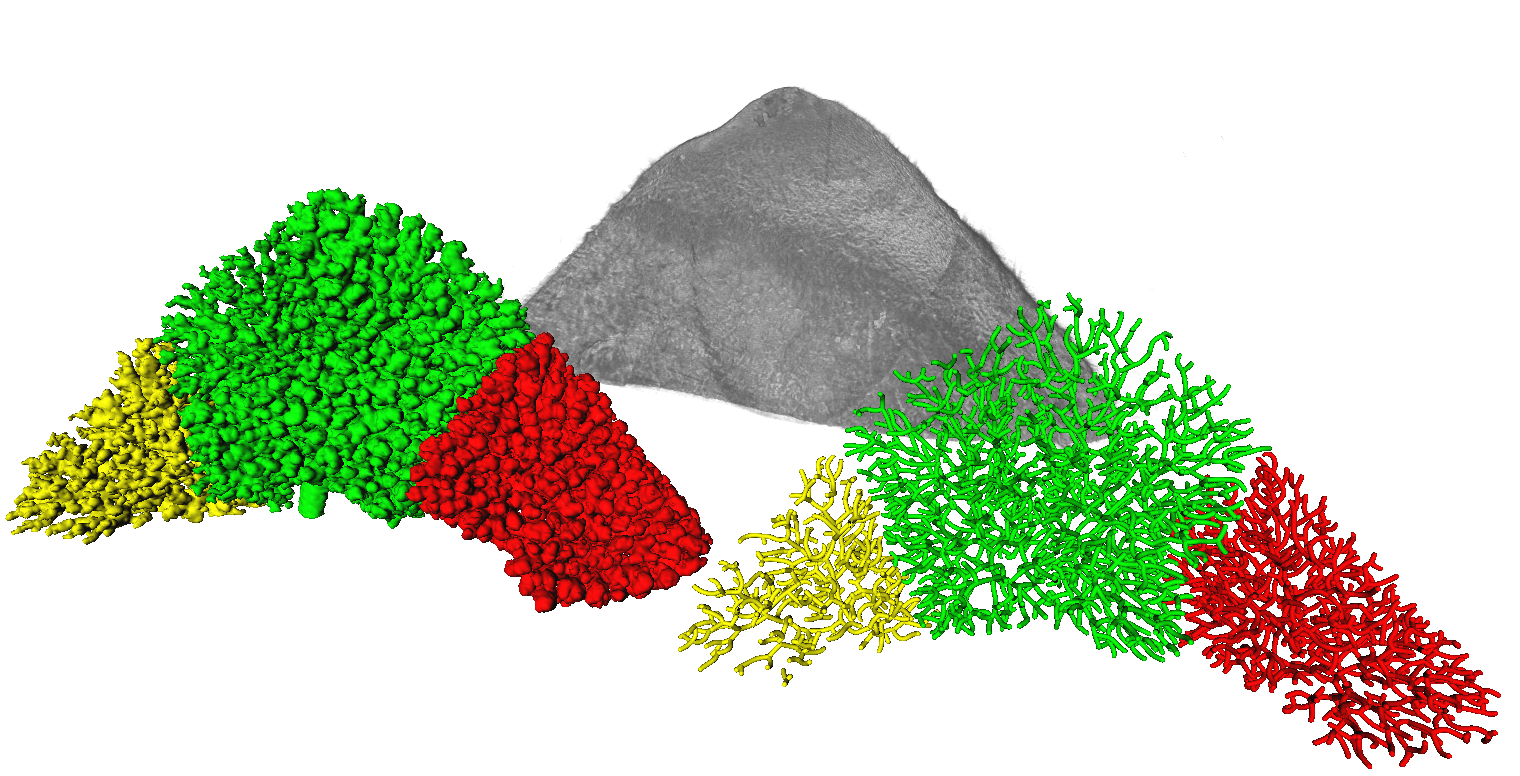
\includegraphics[width=\imagewidth]{img/widefieldscanning/R108C04C-skeleton-merge}};
	   	\draw[|-|,thick] (13,512) -- (705,572) node [midway,right] {\SI{3.8444}{\milli\meter}}; 
	    % 695 px = 3.844 mm > 100 px = 554 um > 90 px = 500um
		\draw[|-|,thick] (\x,\y) -- (180+\x,\y) node [midway,above] {\SI{1}{\milli\meter}}; 
	\end{tikzpicture}%
		\caption{Three dimensional visualization of the distal-medial edge of the right lower lung lobe of a Sprague Dawley rat (same sample as in figure~\ref{fig:FOV increase overview} and~\ref{fig:FOV increase segments}), including the airway skeletons of the extracted airways.}%
	\label{fig:skel}%
\end{figure}